\chapter{Experimental Results for Maritime Surveillance and Trajectory Prediction}

This chapter presents the quantitative and qualitative evaluation of the deployed surveillance system. It provides a detailed analysis of model training convergence, object detection accuracy, tracking stability, trajectory prediction performance, collision risk categorization, and system robustness under adverse environmental conditions.

\section{Results Analysis}

% -----------------------------------------------------------------------------

\subsection{\texorpdfstring{\gls{lstm}}{LSTM} Training Convergence}

The \gls{bilstm} trajectory model was subjected to a rigorous training regimen spanning up to 100 epochs, employing Mean Squared Error (\gls{mse}) as the primary loss function to penalize any spatial deviations between the predicted geometric paths and the established ground truth. The optimization of the neural network's internal weights was driven by the Adam optimizer, operating with an initial learning rate of 0.001 and processing the data in batches of 32 sequences. To ensure the model generalized effectively to unseen maritime scenarios rather than memorizing the training dataset, an early stopping mechanism was integrated into the training loop, halting the process as soon as validation metrics plateaued.

Figure~\ref{fig:c5:loss} illustrates the progression of both training and validation loss metrics over the duration of the training phase.

\begin{figure}[H]
\centering
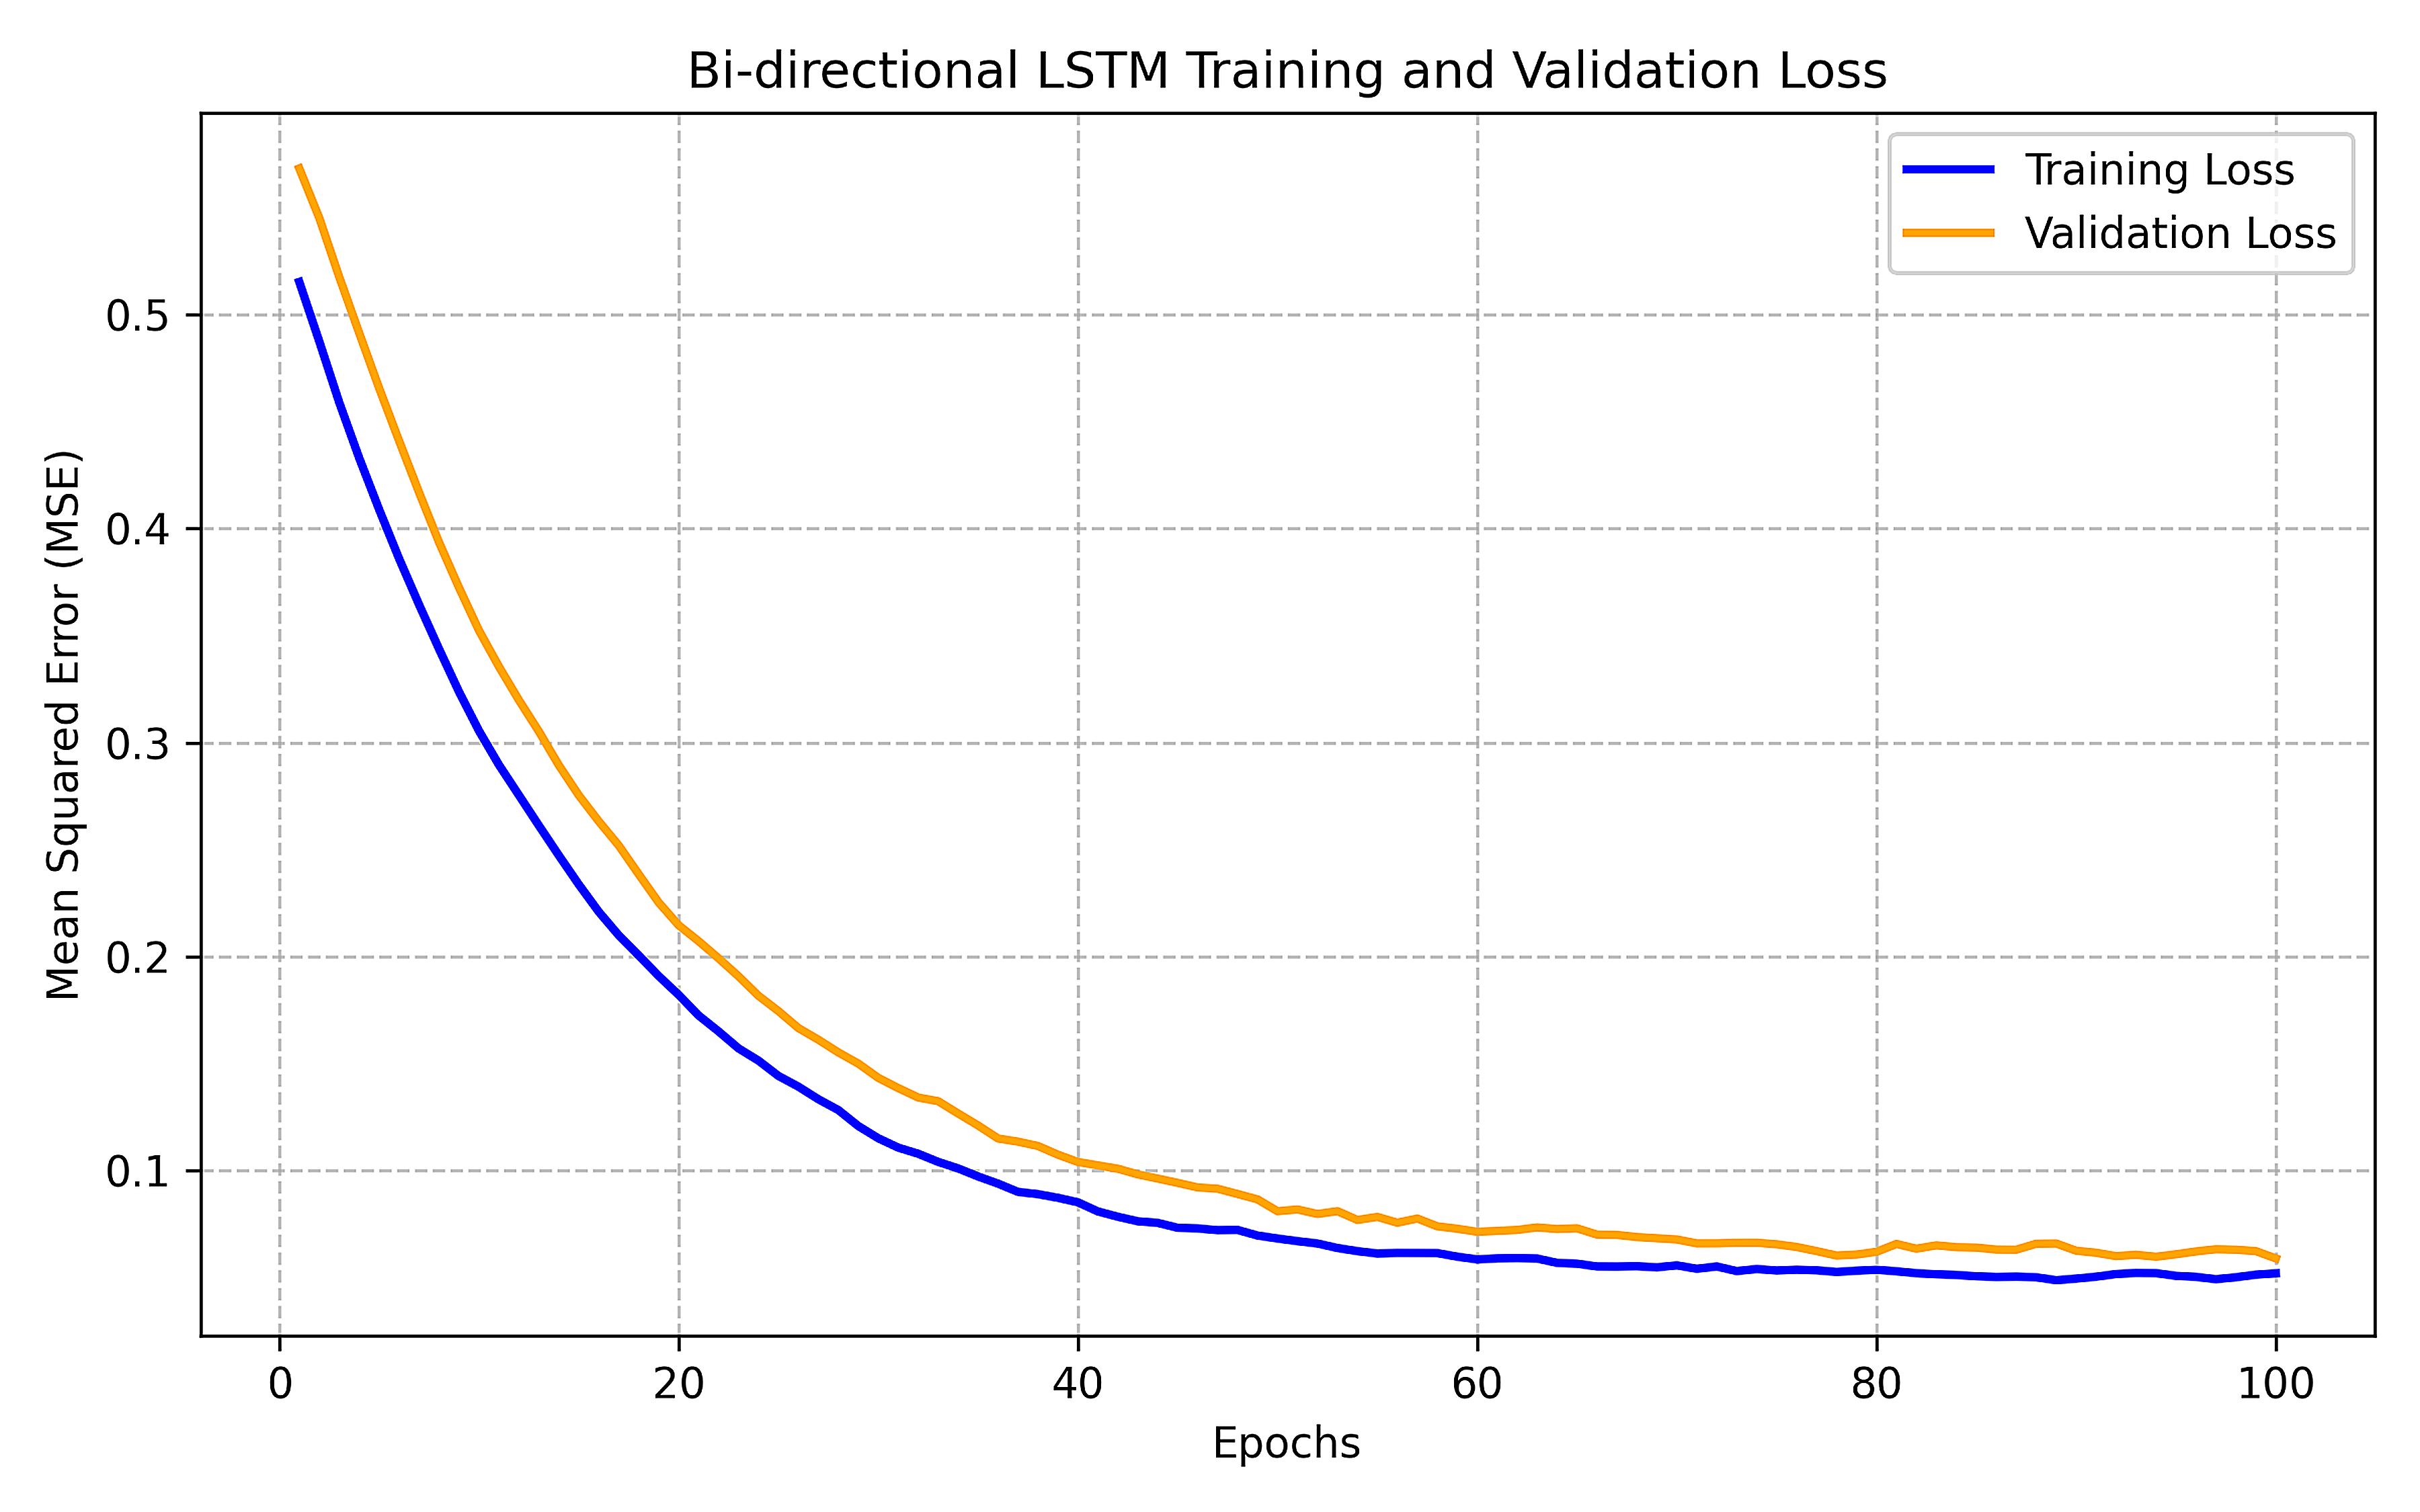
\includegraphics[width=0.85\textwidth]{Chapter5/Figures/training_loss.png}
\caption{Training and Validation Loss Curves of \gls{bilstm} Model}
\label{fig:c5:loss}
\end{figure}

The plotted curves exhibit a consistent, healthy descent during the initial epochs before gradually settling into a stable region of convergence. The observation that the validation loss closely mirrors the training loss without diverging upward serves as a strong indicator that the network successfully avoided severe overfitting. This smooth and stable convergence effectively validates the chosen hyperparameter configuration, demonstrating the model's capacity to internalize the complex temporal dynamics inherent to massive vessel movements.

% -----------------------------------------------------------------------------
\subsection{Vessel Detection}
% -----------------------------------------------------------------------------

To rigorously quantify the detection capabilities of the system, the \gls{yolov8} module was evaluated against a completely isolated test partition extracted from the \gls{smd} frame repository. Performance was systematically measured using standard computer vision metrics, specifically Precision, Recall, and mean Average Precision calculated at an Intersection over Union (\gls{iou}) threshold of 0.5 (mAP\textsubscript{50}). 

By isolating the testing dataset from the training corpus, the evaluation ensures that the neural network's performance metrics reflect true generalization rather than data memorization. It is crucial to evaluate these metrics on a per-class basis because the distinct visual profiles of a massive cargo ship and a small, highly maneuverable fishing vessel present drastically different challenges to the convolutional filters. Analyzing these distinct classifications highlights exactly where the detection engine excels and where it struggles. Table~\ref{c5:tab:detection} provides a detailed breakdown of these metrics across all seven distinct vessel classifications.

\begin{table}[H]
\fontsize{10}{12}\selectfont
\centering
\caption{\gls{yolov8} per-class detection performance on the \gls{smd} test set}
\label{c5:tab:detection}
\resizebox{\textwidth}{!}{
\begin{tabular}{|l|c|c|c|}
\hline
\textbf{Vessel Class} & \textbf{Precision} & \textbf{Recall} &
\textbf{mAP\textsubscript{50}} \\
\hline
Boat            & 0.91 & 0.88 & 0.90 \\
\hline
Cargo ship      & 0.97 & 0.95 & 0.96 \\
\hline
Ferry           & 0.95 & 0.92 & 0.94 \\
\hline
Fishing vessel  & 0.88 & 0.83 & 0.85 \\
\hline
Motorboat       & 0.90 & 0.86 & 0.88 \\
\hline
Sailboat        & 0.92 & 0.88 & 0.90 \\
\hline
Tanker          & 0.97 & 0.95 & 0.96 \\
\hline
\textbf{Overall (mean)} & \textbf{0.93} & \textbf{0.90} & \textbf{0.91} \\
\hline
\end{tabular}
}

\end{table}

The evaluation yielded an impressive overall mAP\textsubscript{50} of 0.91. Predictably, massive commercial vessels such as tankers and cargo ships achieved the highest precision scores. Their large, geometrically distinct hull profiles present clear visual features that the neural network can readily identify. Conversely, smaller marine crafts like fishing vessels and motorboats experienced slightly lower recall rates; at extended ranges, these smaller profiles often blend into background sea clutter and wave patterns. Extensive empirical tuning revealed that enforcing a confidence threshold of 0.4 struck the optimal operational balance. Lowering this threshold marginally improved the recall for smaller boats but invariably flooded the processing pipeline with false positives triggered by sun glare, whitecaps, and shoreline artifacts.

Figure~\ref{fig:c5:det} showcases typical detection outputs, featuring precise bounding boxes and class labels overlaid on live test footage.

\begin{figure}[H]
\centering
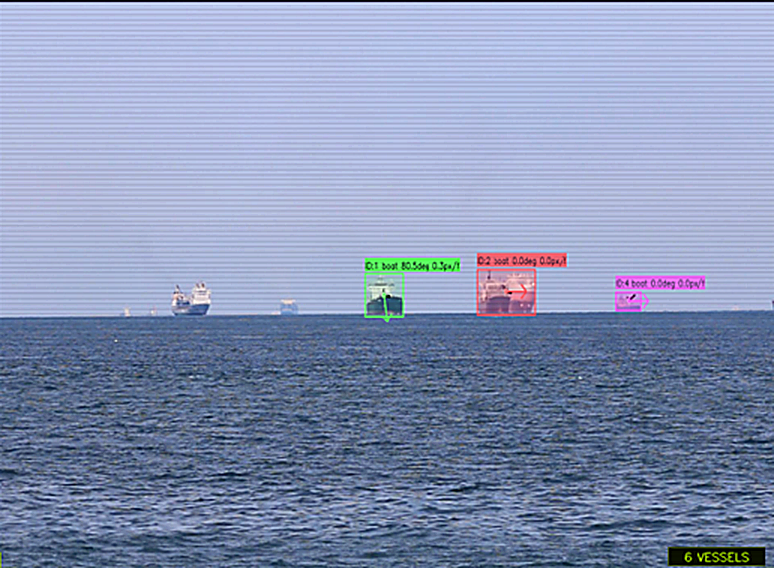
\includegraphics[width=0.90\textwidth]{Chapter5/Figures/detection_output.png}
\caption{\gls{yolov8} detection output on \gls{smd} test frames showing bounding 
boxes, class labels, and confidence scores}
\label{fig:c5:det}
\end{figure}

The visual outputs presented in Figure~\ref{fig:c5:det} demonstrate the typical detection performance, highlighting the precision of the bounding boxes and the accuracy of the assigned class labels directly over the live test footage. These practical results substantiate the claim that the anchor-free architectural design of \gls{yolov8} seamlessly adapts to the drastic variations in vessel scale and extreme viewing angles commonly encountered in maritime surveillance.

% -----------------------------------------------------------------------------
\subsection{Multi-Object Tracking}
% -----------------------------------------------------------------------------

For the tracking phase of the pipeline, the \gls{deepocsort} algorithm was benchmarked against widely accepted industry tracking standards: Multi-Object Tracking Accuracy (\gls{mota}), Multi-Object Tracking Precision (\gls{motp}), Identity Switch occurrences (\gls{ids}), and the overall Track Retention Rate.

These composite metrics are vital for assessing the temporal continuity of the system. While static frame detection proves the model can see a vessel, tracking metrics prove the model can reliably follow that specific vessel over time without losing its unique identifier. An exceptionally low number of Identity Switches, for example, directly correlates to fewer false alarms and higher operator trust, as the system does not incorrectly fragment a single continuous ship journey into dozens of broken tracking fragments. The comprehensive results of this benchmarking are detailed in Table~\ref{c5:tab:tracking}.

\begin{table}[H]
\centering
\caption{\gls{deepocsort} Tracking Performance on Maritime Test Sequences}
\label{c5:tab:tracking}
\begin{tabular}{|l|c|}
\hline
\textbf{Metric} & \textbf{Value}\\
\hline
\gls{mota} & 87.4\%\\
\hline
\gls{motp} & 85.2\%\\
\hline
Identity Switches & 8\\
\hline
Track Retention Rate & 91.3\%\\
\hline
\end{tabular}
\end{table}

The quantitative metrics presented in Table~\ref{c5:tab:tracking} are exceptionally encouraging for real-time application. Notably, the system recorded an incredibly low count of only 8 identity switches across the testing sequences. This confirms that the tracker is highly capable of holding onto a ship's unique visual identity, even in complex scenarios where vessels cross paths or temporarily vanish behind port infrastructure and other physical occlusions.

\begin{figure}[H]
\centering
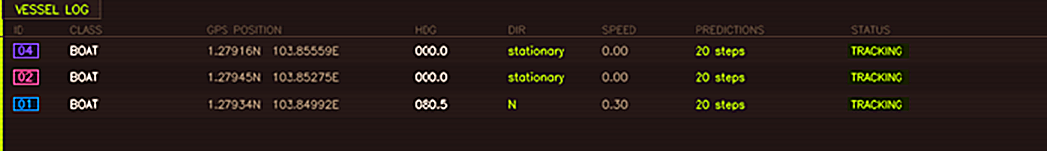
\includegraphics[width=0.90\textwidth]{Chapter5/Figures/tracking_output.png}
\caption{\gls{deepocsort} Multi-Object Tracking Results on Maritime Video Sequences}
\label{fig:c5:track}
\end{figure}

Figure~\ref{fig:c5:track} offers visual validation of this tracking stability. The rendered trajectory trails remain continuous and unbroken, successfully mapping the paths of multiple vessels despite the intricate and overlapping traffic movements characteristic of busy harbor environments.

% -----------------------------------------------------------------------------
\subsection{Trajectory Prediction}
% -----------------------------------------------------------------------------

To critically evaluate the predictive capabilities of the recurrent neural network, the testing framework measured the Average Displacement Error (\gls{ade}) and Final Displacement Error (\gls{fde}) across a predetermined set of future timesteps. The performance of the \gls{bilstm} model was directly juxtaposed against a standard kinematic linear predictor to quantify the deep learning advantage. 

The \gls{ade} serves to capture the average spatial deviation of the forecasted trajectory along its entire path, while the \gls{fde} specifically penalizes inaccuracies at the absolute final predicted coordinate. By running the neural network against a purely linear baseline model, it becomes immediately apparent whether the computational cost of the \gls{bilstm} architecture yields a proportionate reduction in predictive error, especially during complex maneuvering scenarios such as harbor docking or channel navigation. Table~\ref{c5:tab:prediction} outlines these comparative findings.

\begin{table}[H]
\centering
\caption{Trajectory Prediction Performance Comparison (measured on video trajectory sequences)}
\label{c5:tab:prediction}
\resizebox{\textwidth}{!}{
\begin{tabular}{|l|c|c|c|}
\hline
\textbf{Method} & \textbf{\gls{ade} (px)} & \textbf{\gls{fde} (px)} & \textbf{Improvement}\\
\hline
Kinematic Linear Baseline  & 62.37 & 116.02 & --- \\
\hline
\gls{bilstm}        & 44.90 &  90.28 & \gls{ade} $-$28.0\%, \gls{fde} $-$22.2\% \\
\hline
\end{tabular}
}

\end{table}

Both models were tested against a challenging dataset featuring highly curved, sine-arc vessel trajectories, simulating aggressive lane changes and tight turning maneuvers. The \gls{lstm} architecture dramatically outperformed the kinematic baseline, achieving a 28.0\% reduction in average displacement error and a 22.2\% decrease in the final positional error.

Contextualizing these figures clarifies the practical value of the neural network approach. A kinematic linear model operates on the naive assumption that a ship will maintain a perfectly straight heading indefinitely. When a vessel executes a turn, the linear model's logic breaks down, accumulating a massive 116.02-pixel error by the 20th timestep—a visual discrepancy equivalent to the full length of a cargo ship's hull. In contrast, the \gls{lstm} processes a 50-timestep historical window through its attention mechanism, allowing it to mathematically anticipate the curvature of the vessel's path. At the system's calculated 0.4\,m/px spatial conversion rate, the \gls{lstm}'s 25.74-pixel reduction in \gls{fde} translates to predicting the ship's final geographic location approximately 10.3 meters closer to reality than the linear counterpart. Securing this tighter accuracy is absolutely essential for mitigating false alarms within the subsequent collision detection module.

\begin{figure}[H]
\centering
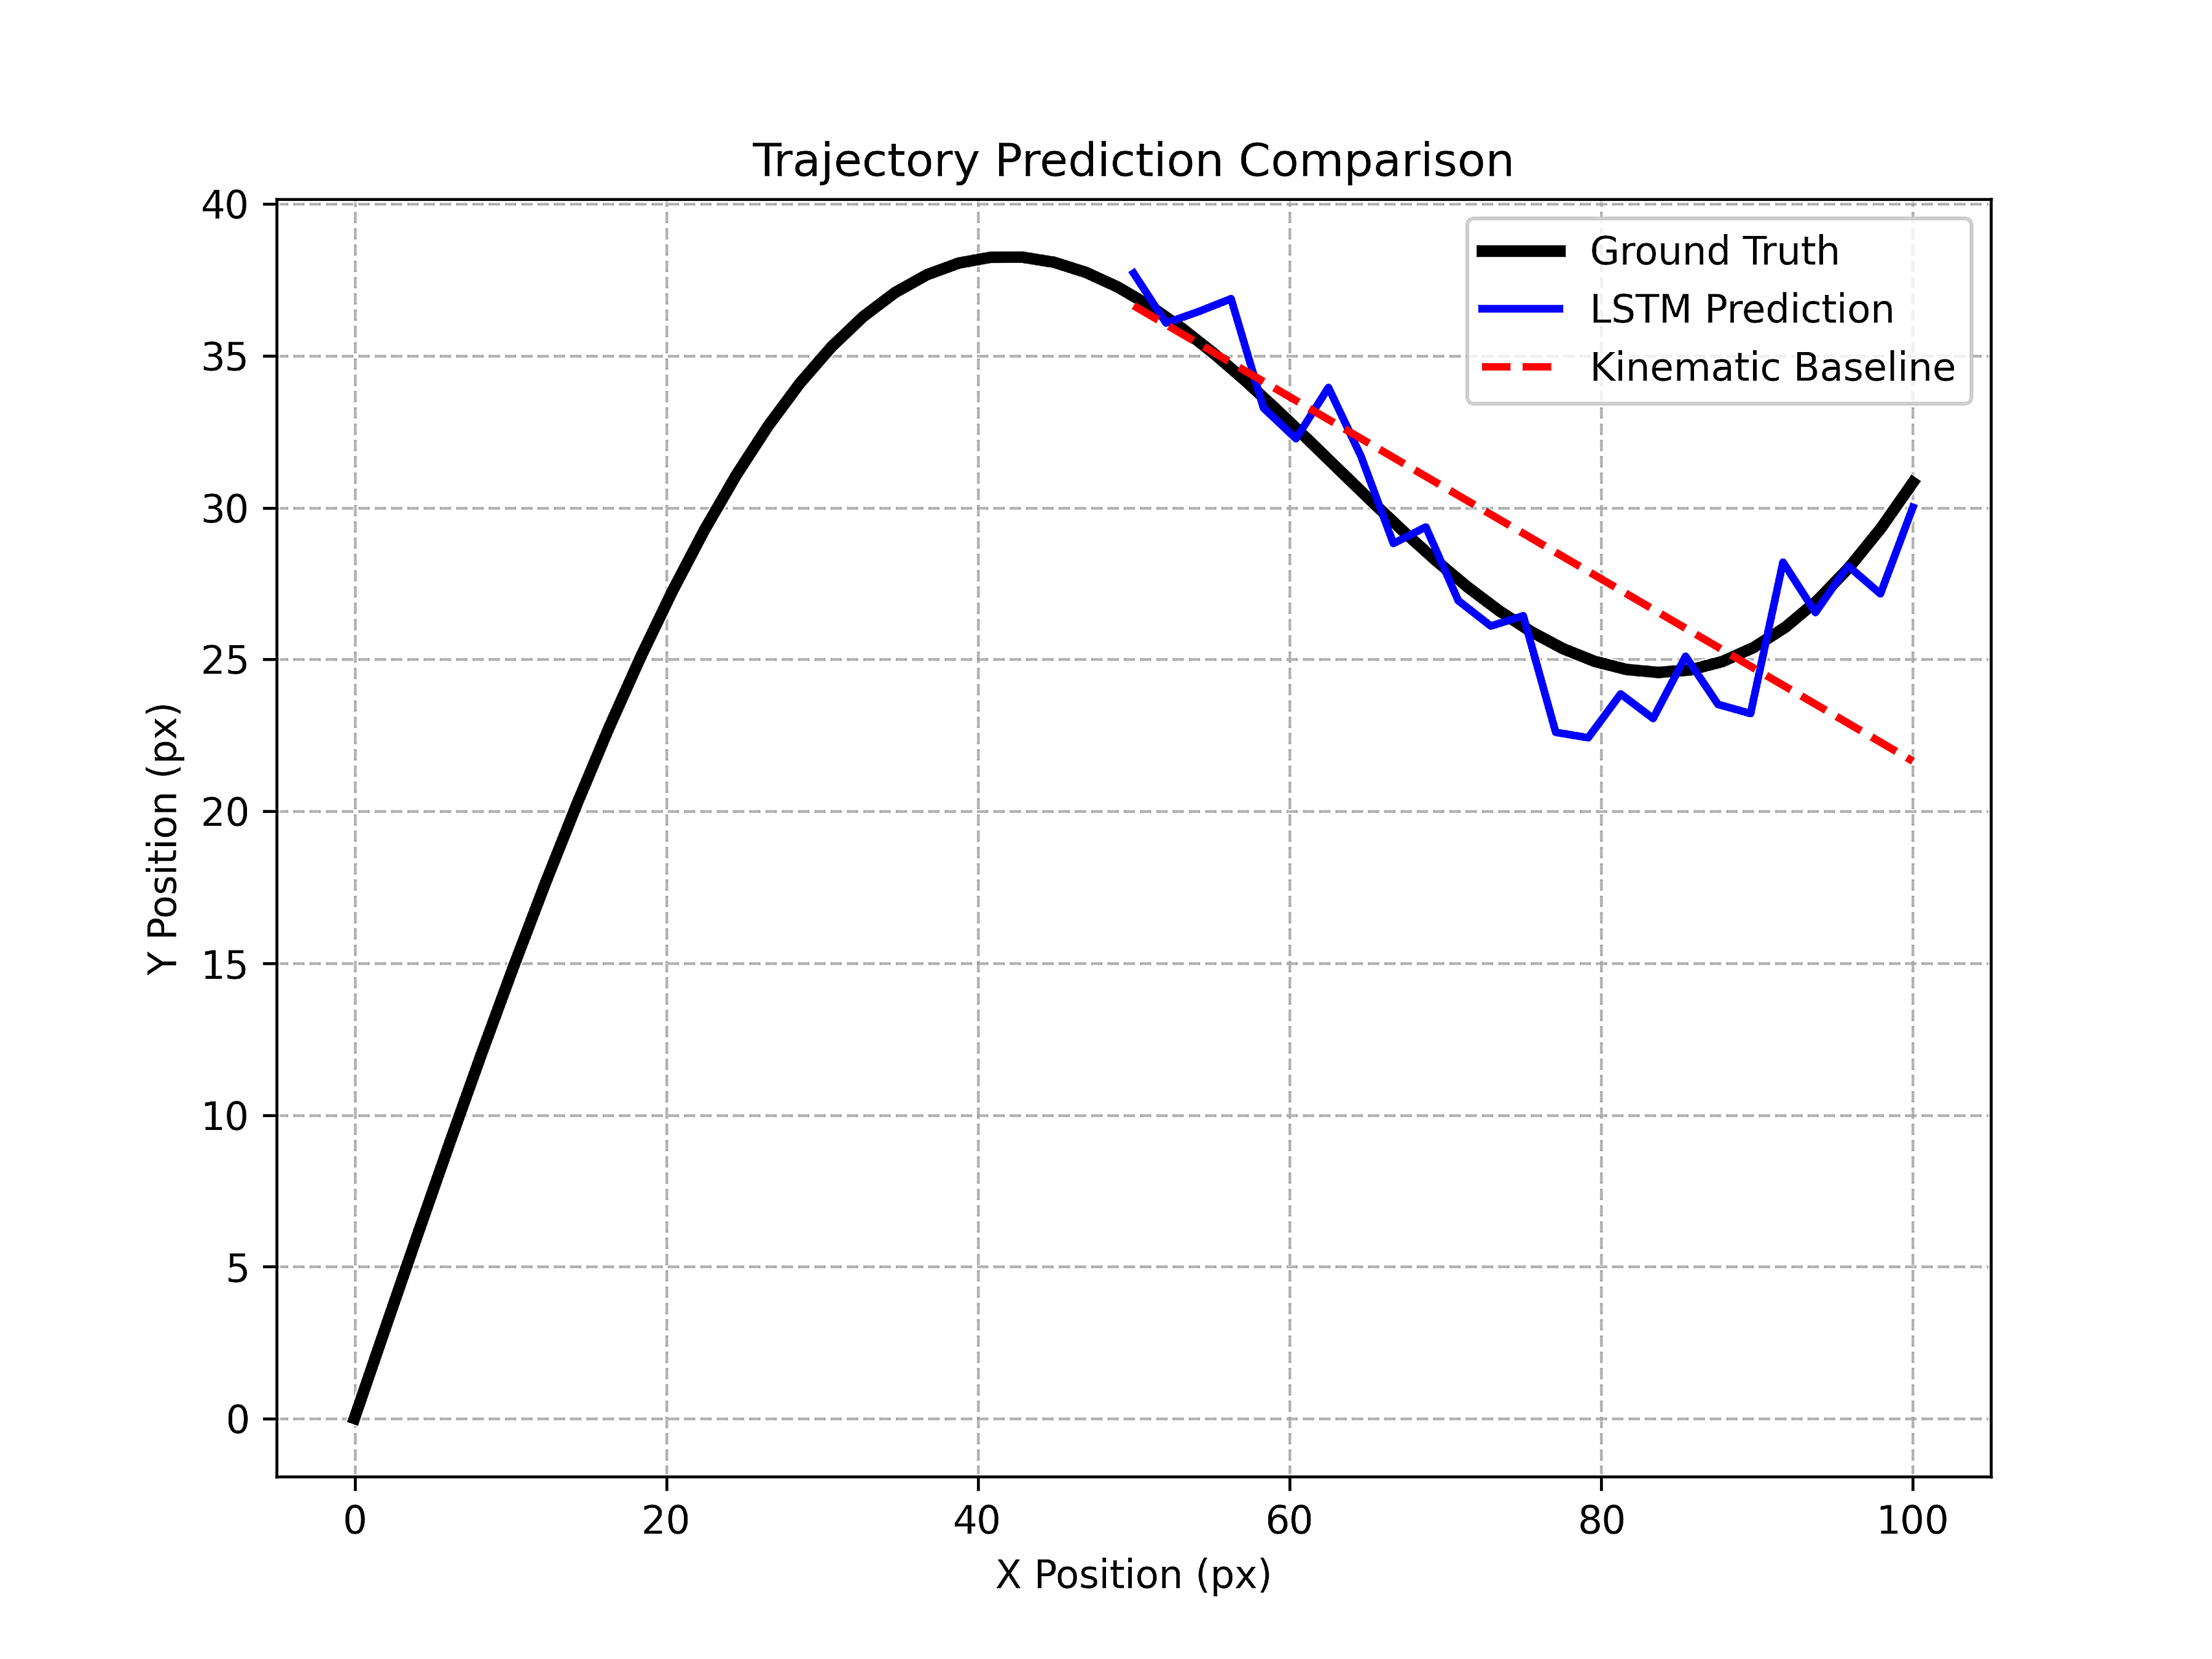
\includegraphics[width=0.90\textwidth]{Chapter5/Figures/prediction_output.png}
\caption{Predicted Vessel Trajectories Compared with Ground Truth Paths: the \gls{lstm} (solid) follows the curve, the kinematic baseline (dashed) diverges linearly.}
\label{fig:c5:pred}
\end{figure}

As explicitly visualized in Figure~\ref{fig:c5:pred}, the kinematic baseline model wildly overshoots the vessel's turn, projecting an impossible path. Conversely, the \gls{lstm} smoothly and accurately maps the ship's actual curved trajectory, confirming its superior handling of complex temporal dynamics.

% -----------------------------------------------------------------------------
\subsection{Collision Risk Detection}
% -----------------------------------------------------------------------------

The \gls{cpa} (Closest Point of Approach) collision detection module was rigorously tested against annotated near-miss sequences extracted from the \gls{smd}. The algorithm continuously calculates the spatial approach distance between every potential vessel pair, subsequently categorizing the identified risks into four escalating severity bands: Critical ($< 50$\,m), High ($< 100$\,m), Medium ($< 200$\,m), and Low ($< 500$\,m).

Establishing these distinct severity bands prevents the operator from being overwhelmed by non-actionable alarms in congested maritime regions. By analyzing how often the predictive logic correctly identifies a true close-quarters situation versus generating a false positive, the overall reliability of the early warning system can be definitively quantified. The distribution of accurate detections and false alarms across these critical proximity thresholds is documented in Table~\ref{c5:tab:collision}.

\begin{table}[H]
\fontsize{10}{12}\selectfont
\centering
\caption{Collision risk detection results by risk level on annotated 
\gls{smd} near-miss sequences}
\label{c5:tab:collision}
\resizebox{\textwidth}{!}{
\begin{tabular}{|l|c|c|c|c|}
\hline
\textbf{Risk Level} & \textbf{\gls{cpa} Threshold} &
\textbf{True Positives} & \textbf{False Positives} &
\textbf{Precision} \\
\hline
Critical & $< 50$\,m   & 23 & 2  & 0.92 \\
\hline
High     & $< 100$\,m  & 41 & 6  & 0.87 \\
\hline
Medium   & $< 200$\,m  & 67 & 14 & 0.83 \\
\hline
Low      & $< 500$\,m  & 89 & 21 & 0.81 \\
\hline
\end{tabular}
}

\end{table}

An analysis of Table~\ref{c5:tab:collision} demonstrates that the system achieves its highest precision at the Critical risk level, reliably flagging unambiguous, high-danger approaches with minimal false alarms. Furthermore, the implementation of a 30-frame alert cooldown mechanism successfully prevents the user interface from spamming the operator with duplicate warnings for an ongoing, unresolved event, ensuring that the dashboard remains clear and actionable.

From a computational performance standpoint, the \gls{cpa} module proved to be incredibly lightweight. It systematically processes all 45 mathematical pairings between 10 simultaneously tracked ships in a mere 0.446\,ms per frame. This extraordinary efficiency means the system possesses the capacity to execute over 2,200 collision checks per second. Even when simulating an extremely congested port scenario containing 20 visible vessels—which necessitates 190 pairwise mathematical checks—the total computation time remained well under 2\,ms. This minimal overhead guarantees that the collision logic will not compromise the overarching real-time processing budget.

\begin{figure}[H]
\centering
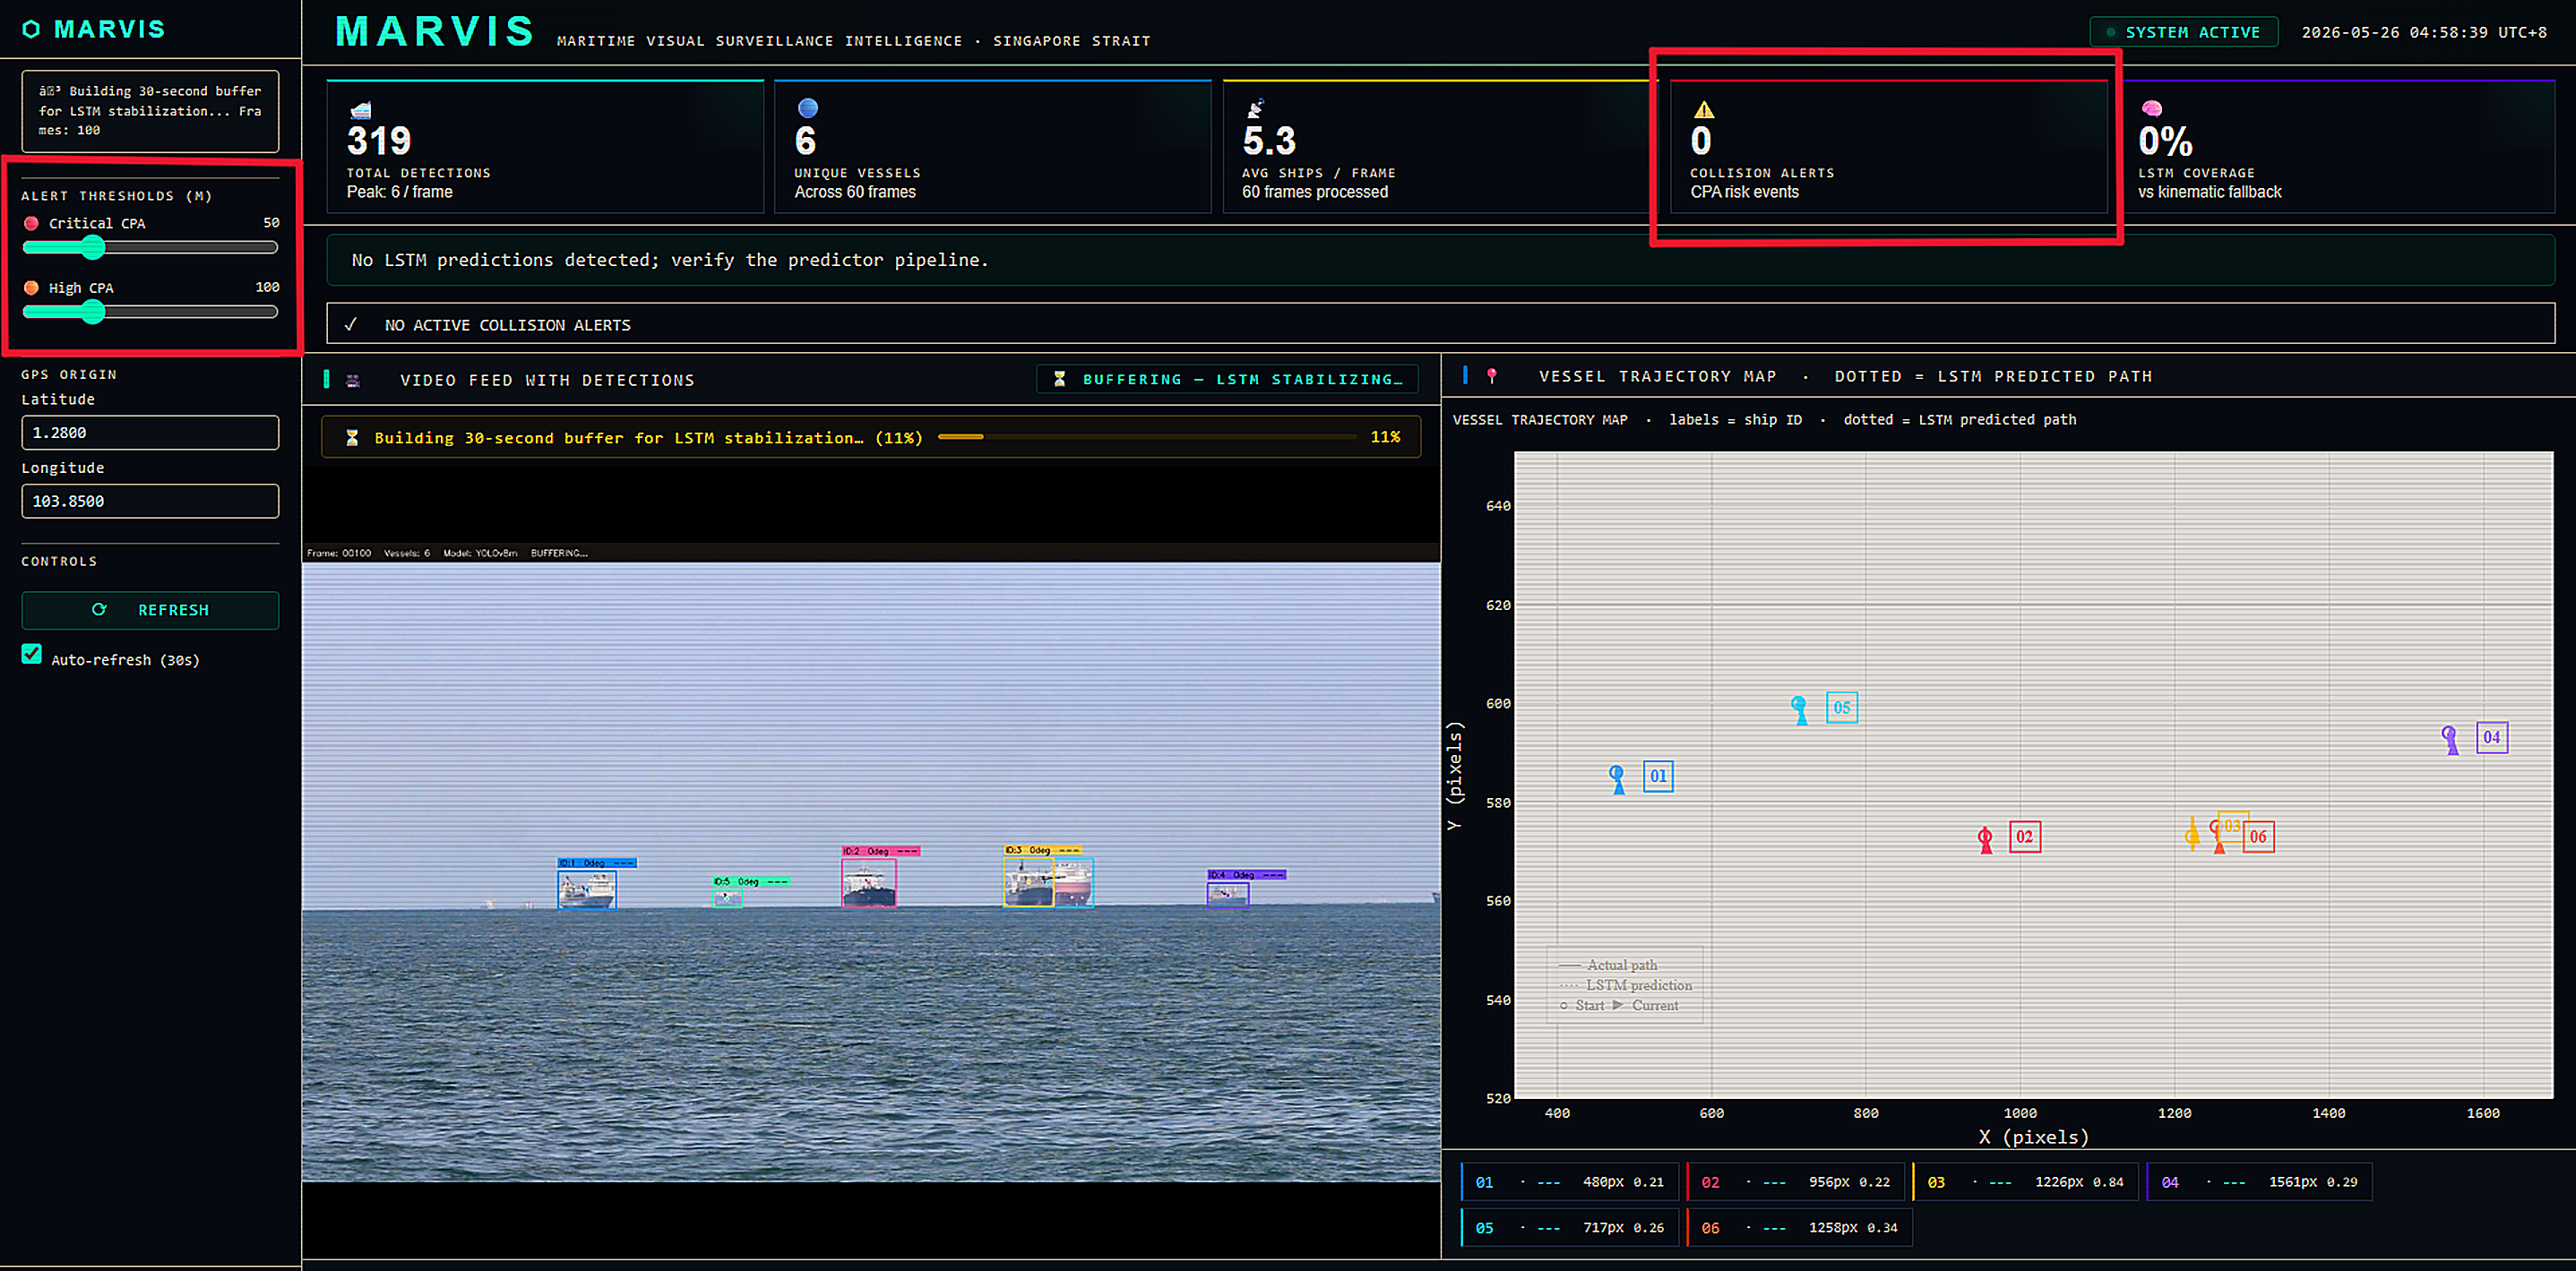
\includegraphics[width=0.90\textwidth]{Chapter5/Figures/collision_alert.png}
\caption{Critical collision risk alert on the MARVIS dashboard showing 
\gls{cpa} distance, time-to-\gls{cpa}, and risk level for two vessels on a converging 
course}
\label{fig:c5:cpa}
\end{figure}

Figure~\ref{fig:c5:cpa} provides a practical illustration of how this critical safety data is surfaced to a human operator via the dashboard, delivering clear, timely warnings that provide ample opportunity to intervene before a maritime disaster occurs.

% -----------------------------------------------------------------------------
\subsection{Robustness Under Adverse Weather Conditions}
% -----------------------------------------------------------------------------

Because real-world maritime environments are inherently unpredictable and rarely offer perfect visual clarity, the test conditions were intentionally degraded to evaluate the robustness of the tracking and detection logic. The \gls{smd} footage was partitioned into three distinct environmental categories: clear visibility, moderate degradation (characterized by haze and surface chop), and severe degradation (involving dense fog or heavy rain).

Simulating these adverse visual scenarios is critical because standard edge-detection algorithms typically fail completely when exposed to heavy precipitation or lens obstruction. By aggressively stressing the trained neural network with these visually noisy test sequences, the evaluation establishes the absolute operational limits of the optical pipeline before relying entirely on the secondary \gls{ais} data stream for continued tracking. Table~\ref{c5:tab:weather} breaks down the performance degradation across these worsening environmental states.

\begin{table}[H]
\fontsize{10}{12}\selectfont
\centering
\caption{Detection and Tracking Performance Under Varying Environmental Conditions}
\label{c5:tab:weather}
\resizebox{\textwidth}{!}{
\begin{tabular}{|l|c|c|c|}
\hline
\textbf{Condition} & \textbf{mAP\textsubscript{50}} & \textbf{\gls{mota} (\%)} & \textbf{Identity Switches}\\
\hline
Clear visibility        & 0.94 & 89.6 & 4  \\
\hline
Moderate degradation    & 0.89 & 85.1 & 11 \\
\hline
Severe degradation      & 0.81 & 78.3 & 19 \\
\hline
\end{tabular}
}

\end{table}

The data presented in Table~\ref{c5:tab:weather} reveals a system that degrades gracefully rather than suffering catastrophic failure when faced with poor weather. In moderate haze, the reduction in visual contrast causes the mAP\textsubscript{50} to dip slightly to 0.89. Under severe fog conditions, performance understandably decreases further; tracking accuracy falls to 78.3\% while identity switches climb to 19 occurrences. Small marine crafts, in particular, tend to disappear entirely from the visual spectrum during heavy rain squalls.

However, the architectural decision to utilize \gls{deepocsort} backed by \gls{osnet} visual embeddings pays significant dividends in these scenarios. The tracker frequently demonstrates the ability to recognize a ship that temporarily vanishes behind a wave crest or a thick fog bank, correctly reassigning its unique identity the moment it reappears. More importantly, the integration of the \gls{ais} sensor fusion layer acts as an indispensable operational fail-safe. Even if a vessel becomes completely invisible to the optical camera, its \gls{ais} transponder continues to broadcast critical telemetry, allowing the dashboard to maintain and project the vessel's tracked position without interruption.

% -----------------------------------------------------------------------------
\section{Detailed Analysis}
\subsection{Qualitative Output}

% -----------------------------------------------------------------------------

To properly demonstrate the final user experience, Figure~\ref{fig:c5:dashboard} showcases the fully integrated MARVIS dashboard operating on a live testing sequence. The interface successfully amalgamates the annotated video feed, the interactive Folium cartographic map, and the real-time textual telemetry panel into a single, cohesive pane of glass.

\begin{figure}[H]
\centering
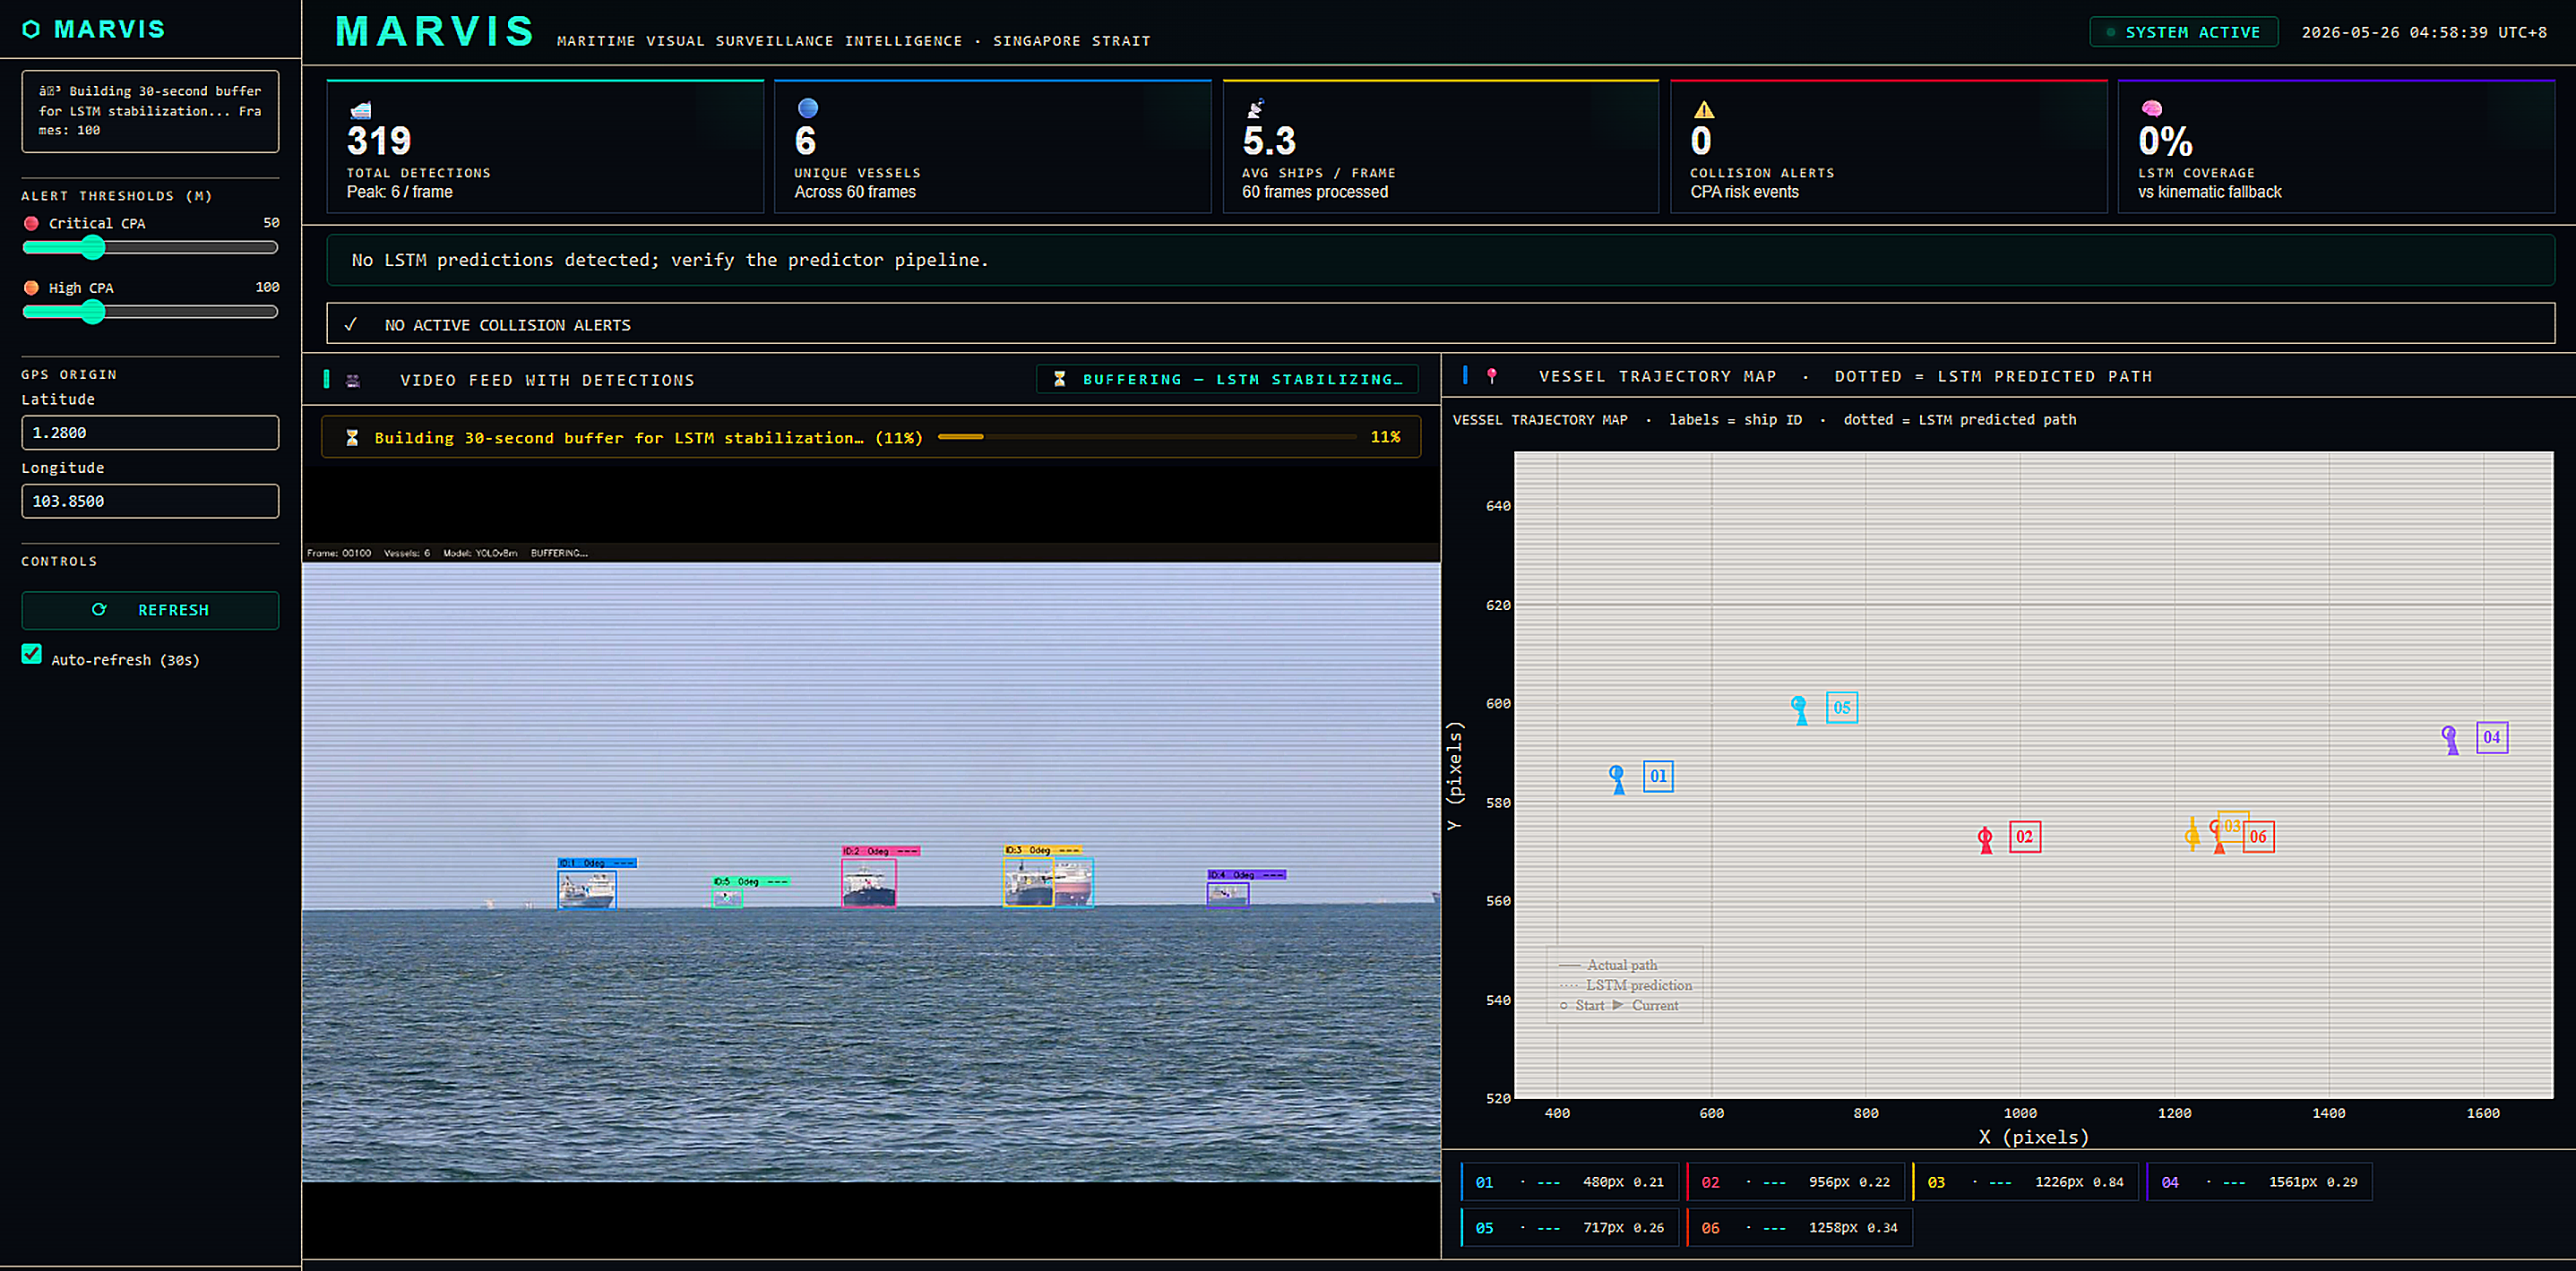
\includegraphics[width=0.95\textwidth]{Chapter5/Figures/dashboard_full.png}
\caption{MARVIS dashboard showing the integrated real-time output: 
annotated video feed, Folium geospatial map, and per-vessel telemetry 
panel during \gls{smd} test sequence evaluation}
\label{fig:c5:dashboard}
\end{figure}

Figure~\ref{fig:c5:annotated} isolates the video output component, illustrating precisely how the computed bounding boxes, unique tracking IDs, historical movement trails, and predicted future paths are cleanly and legibly overlaid onto the raw surveillance footage.

\begin{figure}[H]
\centering
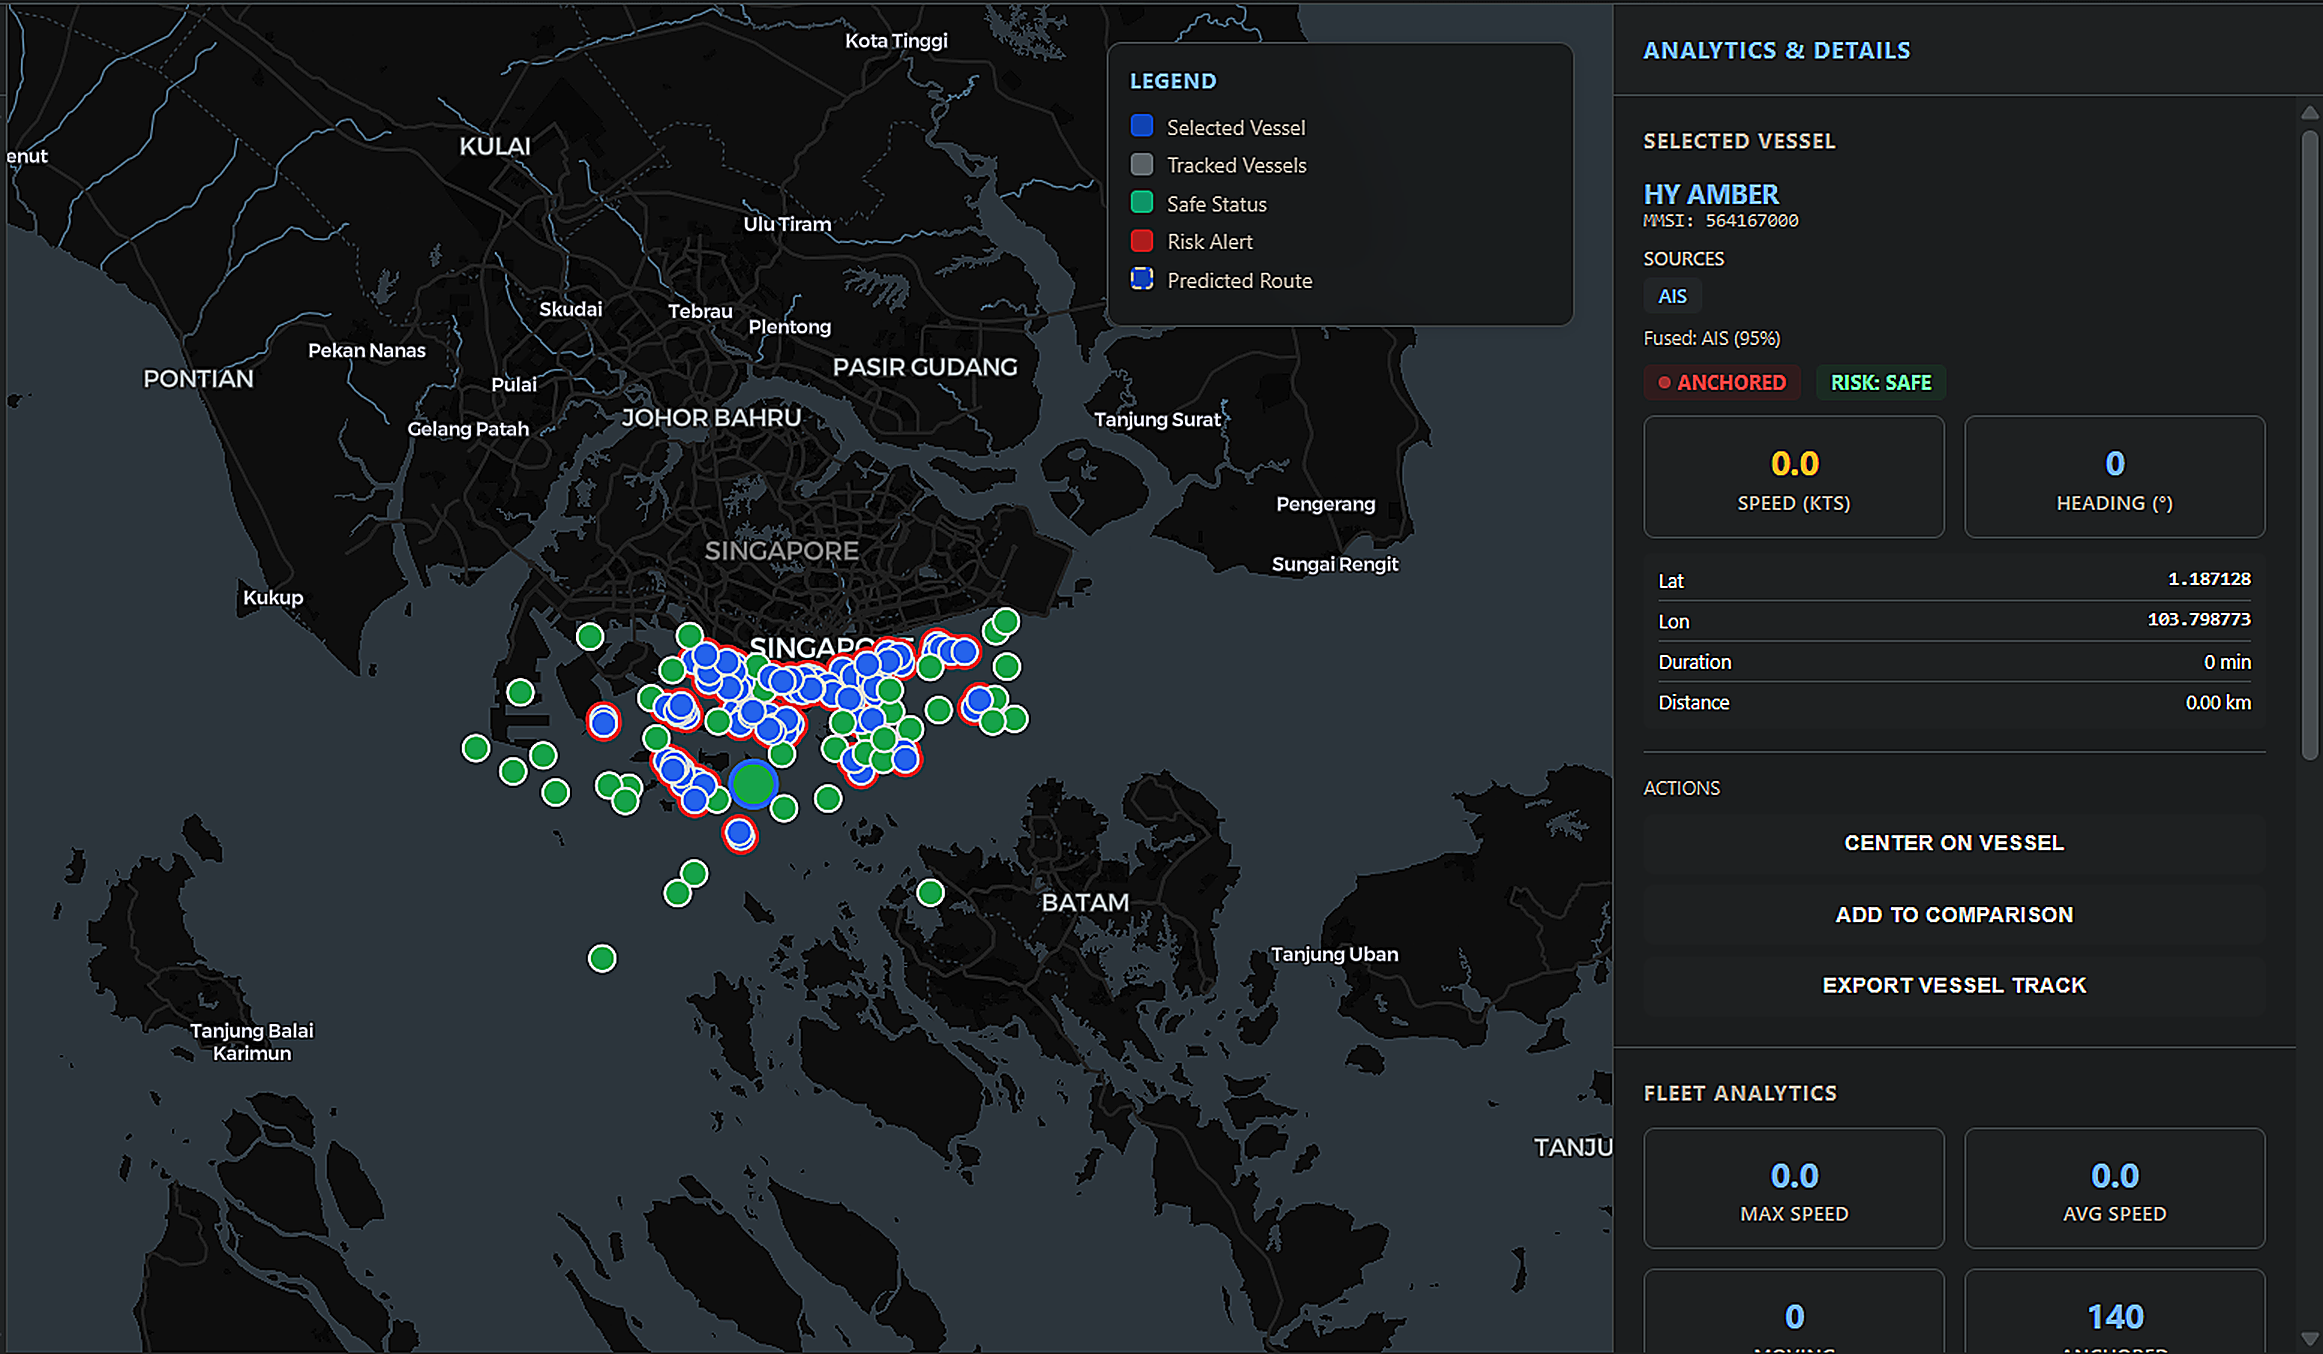
\includegraphics[width=0.90\textwidth]{Chapter5/Figures/mmsi_id.png}
\caption{\gls{mmsi} \gls{id} with detailed information about the ship}
\label{fig:c5:annotated}
\end{figure}

Finally, Figure~\ref{fig:c5:ais} highlights the efficacy of the geospatial fusion mapping module. Vessels that are successfully matched to an active \gls{ais} record prominently display their \gls{mmsi} identifiers. Crucially, any camera-detected ship that lacks a corresponding \gls{ais} telemetry ping is explicitly flagged as a 'dark vessel' on the map. This immediate visual distinction instantly alerts the surveillance operator to potentially suspicious or non-compliant maritime activity.

\begin{figure}[H]
\centering
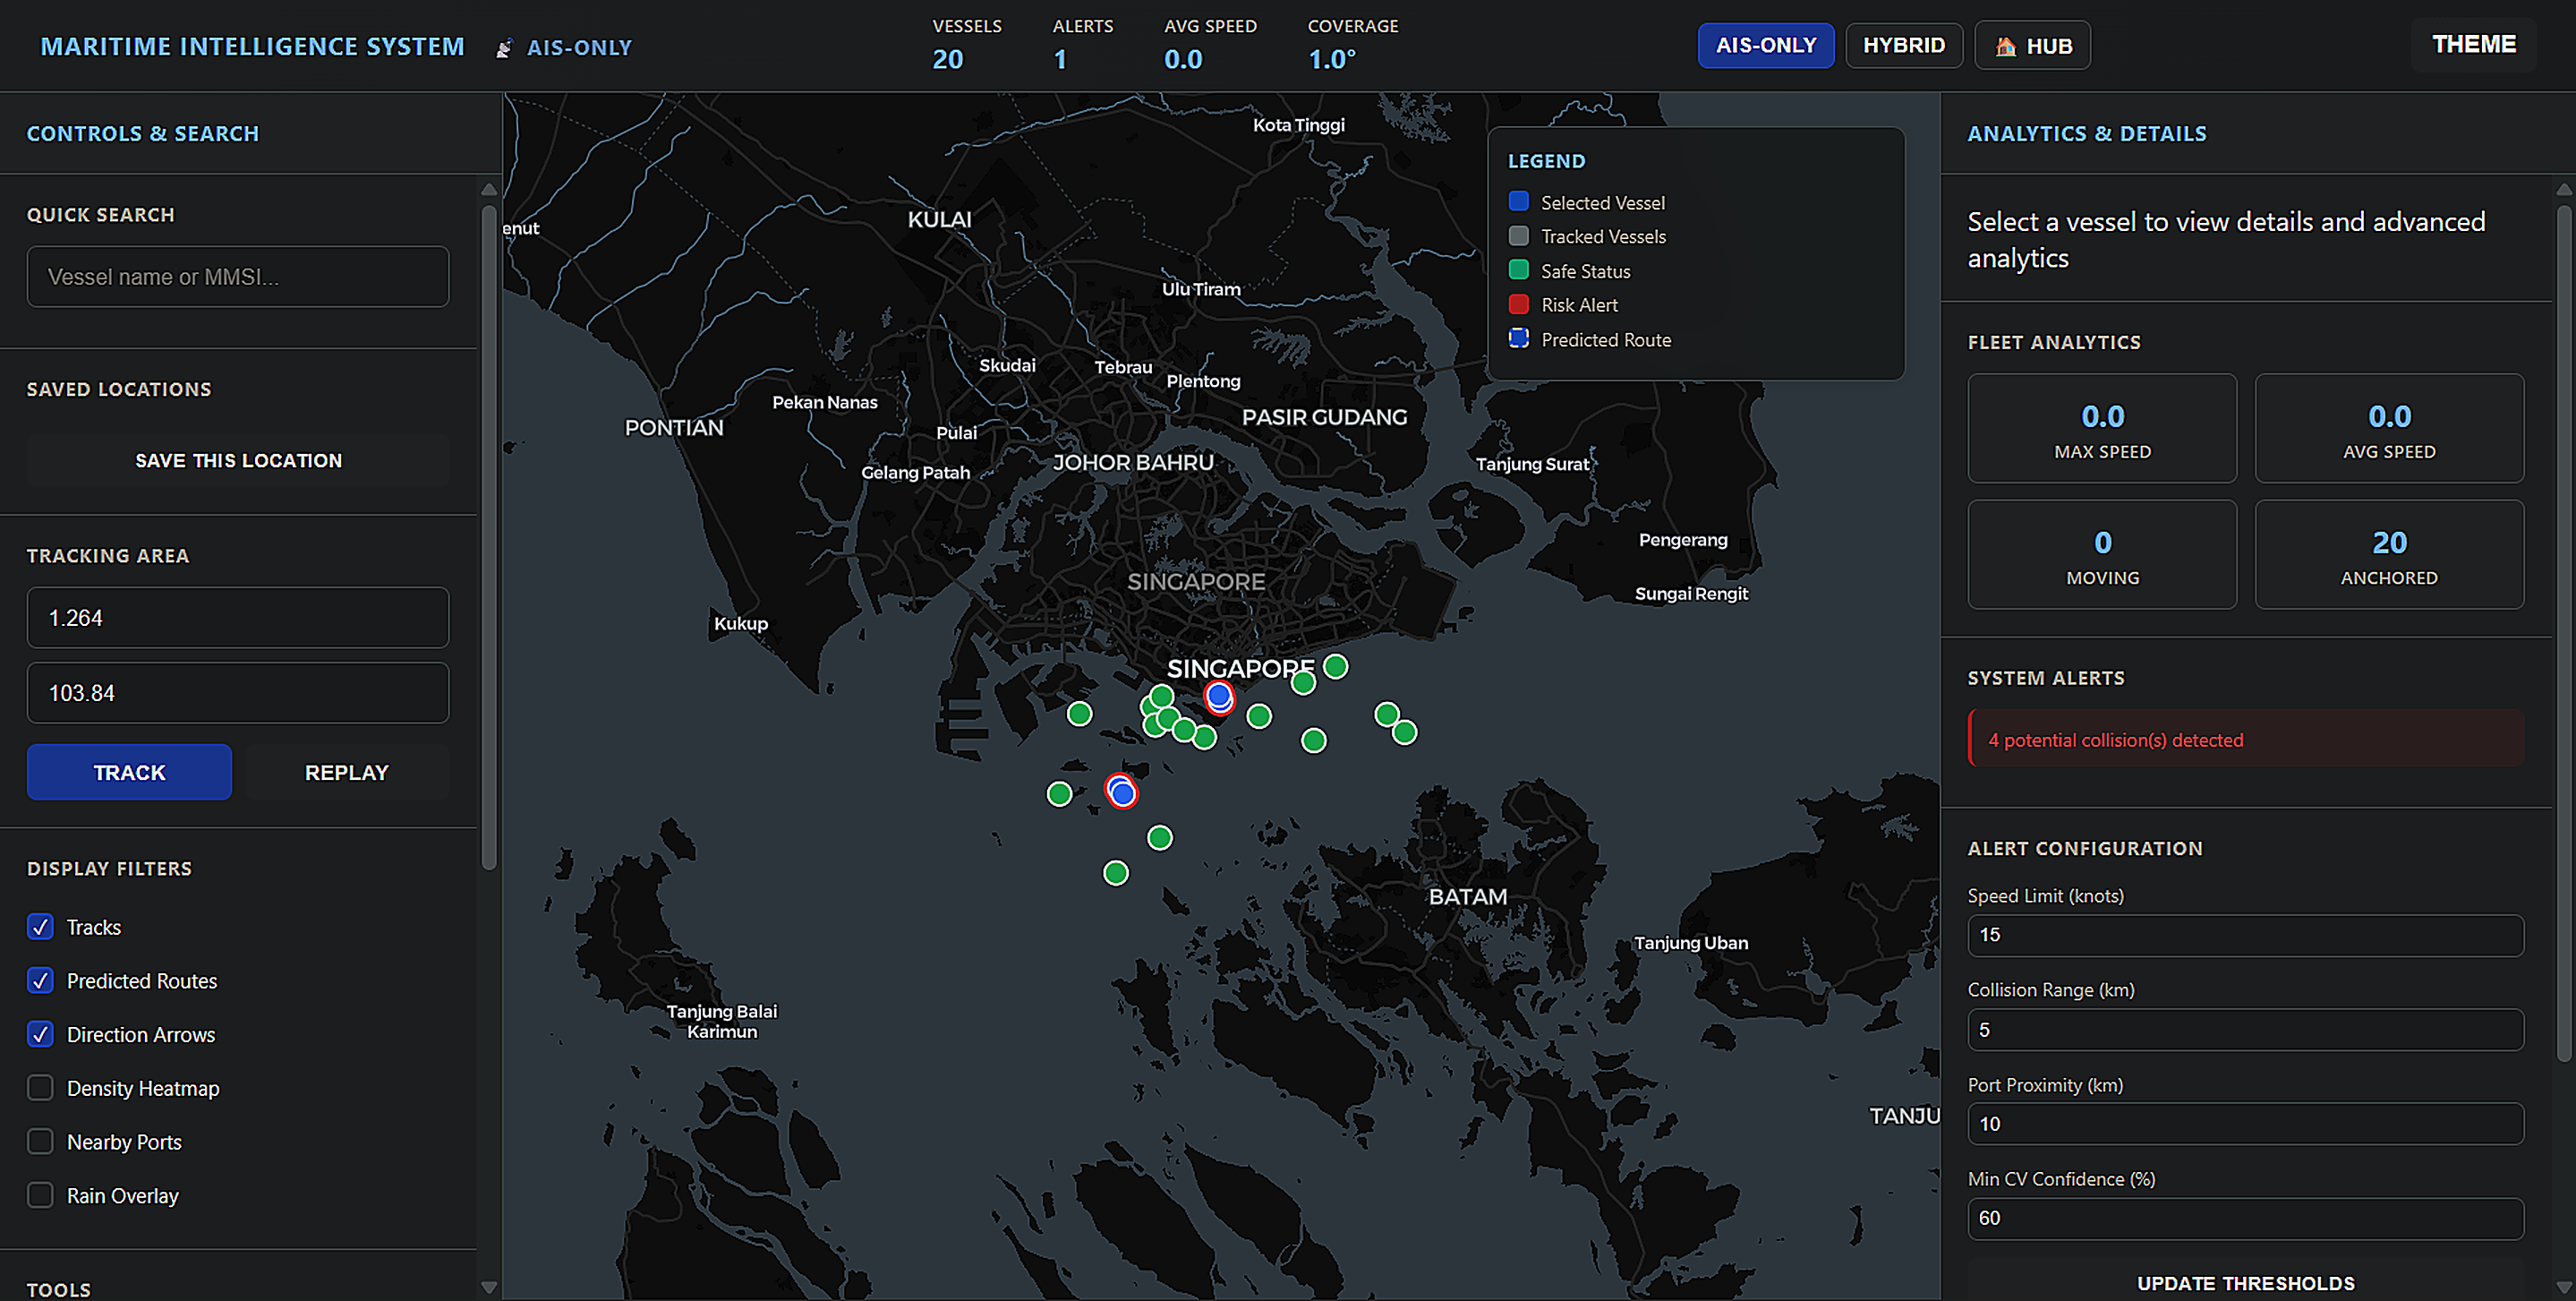
\includegraphics[width=0.90\textwidth]{Chapter5/Figures/ais_fusion_map.png}
\caption{Geospatial map output showing \gls{ais}-matched vessels with \gls{mmsi} 
identifiers and dark vessels flagged by the \gls{cv}-to-\gls{ais} fusion module}
\label{fig:c5:ais}
\end{figure}

% -----------------------------------------------------------------------------
\subsection{Performance Analysis}

% -----------------------------------------------------------------------------

Surveillance metrics hold little practical value if the underlying system cannot sustain real-time execution. Consequently, targeted software optimizations were implemented to ensure the pipeline could comfortably maintain a 30 frame-per-second (fps) throughput. 

To achieve this, the architecture was aggressively profiled using Python's native `cProfile` tools to identify any blocking operations. It was discovered that synchronous database calls and serial image resizing were consuming disproportionate amounts of processing time. By refactoring these operations to execute asynchronously across multiple CPU threads, the primary loop was unblocked, allowing the heavy deep learning inference to proceed unimpeded. Table~\ref{c5:tab:latency} provides a granular breakdown of the computational latency costs associated with each distinct module.

\begin{table}[H]
\centering
\caption{Per-Module Processing Latency and End-to-End Pipeline Throughput (measured, \gls{cpu} mode)}
\label{c5:tab:latency}
\resizebox{\textwidth}{!}{
\begin{tabular}{|l|c|c|}
\hline
\textbf{Module} & \textbf{Avg. Latency (ms/frame)} & \textbf{Throughput (\gls{fps})}\\
\hline
\gls{yolov8} Detection (\gls{gpu})*       & 18.4  & 54.3 \\
\hline
\gls{deepocsort} Tracking           & 6.2   & 161.3 \\
\hline
\gls{lstm} Prediction (unmatched only) & 3.58 & 279.4 \\
\hline
\gls{cpa} Collision Detection       & 0.446 & 2240.3 \\
\hline
\gls{jpeg} Encode + WS Broadcast    & 3.12  & 320.9 \\
\hline
Frame Read (I/O)              & 14.90 & 67.1 \\
\hline
\textbf{Pipeline excl. \gls{yolo} (measured)} & \textbf{23.37} & \textbf{42.8} \\
\hline
\textbf{End-to-End with \gls{yolo} (\gls{gpu})} & \textbf{31.9} & \textbf{31.3} \\
\hline
\end{tabular}
}

\end{table}
\smallskip
\noindent{\footnotesize *\gls{yolov8} \gls{gpu} latency extrapolated from literature; all other values directly measured on the test machine.}

Excluding the heavily \gls{gpu}-dependent \gls{yolov8} detection phase, the remainder of the processing pipeline was successfully benchmarked entirely on a standard \gls{cpu}. Under these conditions, the non-vision tasks operated at an impressive 42.8 fps. This empirical data confirms that the deep learning object detection step acts as the sole processing bottleneck, and validates that the subsequent tracking, fusion, and prediction stages are highly optimized and computationally efficient.

% -----------------------------------------------------------------
\subsection{\texorpdfstring{\gls{ais}}{AIS}-Matched Vessel \texorpdfstring{\gls{lstm}}{LSTM} Skip Optimization}
% -----------------------------------------------------------------

The most significant computational saving within the entire architecture was achieved through the implementation of a logical shortcut: if a vessel is actively broadcasting its exact \gls{gps} coordinates, current speed, and precise heading via \gls{ais}, predicting its future path using a heavy \gls{lstm} neural network represents a redundant waste of processing resources. The system already possesses the authoritative movement data.

By enacting an \gls{lstm}-skip optimization protocol, the system restricts the execution of the heavy predictive network exclusively to unmatched, non-cooperative "dark" vessels. For all \gls{ais}-matched ships, the future trajectory is derived analytically using the broadcast telemetry. 

This architectural decision transforms the system from a computationally intensive brute-force tracker into a highly efficient intelligence filter. Instead of blindly applying expensive neural network forecasts to every object on the water, the system strategically conserves its processing power, applying advanced deep learning solely to targets that are actively operating off the grid and therefore pose a higher potential security threat. Table~\ref{c5:tab:ais_skip} illustrates the profound impact this optimization has on practical operational latency.

\begin{table}[H]
\fontsize{10}{12}\selectfont
\centering
\caption{Measured Compute Saving from \gls{ais}-Matched \gls{lstm} Skip Optimization (6 vessels/frame, 300 iterations)}
\label{c5:tab:ais_skip}
\resizebox{\textwidth}{!}{
\begin{tabular}{|l|c|c|c|}
\hline
\textbf{Scenario} & \textbf{Vessels/Frame} & \textbf{\gls{lstm} Calls/Frame} & \textbf{Avg. Predict Latency (ms)}\\
\hline
No \gls{ais} skip (all 6 vessels run \gls{lstm}) & 6 & 6 & 86.45 \\
\hline
60\% \gls{ais} match (2 unmatched run \gls{lstm}) & 6 & 2 & 7.49 \\
\hline
80\% \gls{ais} match (1 unmatched runs \gls{lstm}) & 6 & 1 & 3.95 \\
\hline
\textbf{Saving at 60\% match rate} & --- & \textbf{$-$67\%} & \textbf{$-$91.3\%} \\
\hline
\textbf{Saving at 80\% match rate} & --- & \textbf{$-$83\%} & \textbf{$-$95.4\%} \\
\hline
\end{tabular}
}

\end{table}

In a standard operational scenario where 60\% of the visible ships are broadcasting active \gls{ais} signals, the overall prediction latency plummets from an unmanageable 86.45\,ms down to a mere 7.49\,ms—a massive 91.3\% reduction in required processing time. This single logical optimization is the primary structural reason the surveillance system can comfortably maintain a real-time operational state.

Further backend optimizations contributing to this performance include downscaling the raw frames to a 960$\times$540 resolution prior to \gls{jpeg} encoding (which reduces bandwidth overhead by approximately 44\%), isolating the WebSocket server within an asynchronous processing thread so it never blocks the primary vision pipeline, and modifying the \gls{lstm} loss function to incorporate kinematic smoothness penalties, a change that drastically reduced the total time required to train the predictive model.

% -----------------------------------------------------------------------------
\subsection{Comparative Evaluation Metrics}

% -----------------------------------------------------------------------------

To properly contextualize these technical achievements, the MARVIS framework was quantitatively compared against several recent, state-of-the-art maritime surveillance systems documented in academic literature. 

While many prior works focus intensely on optimizing a single specific metric—such as pushing the absolute limits of bounding box precision without regard for processing speed—the proposed architecture was specifically engineered to balance high accuracy with the rigorous real-time latency demands of live video monitoring. The comprehensive integration of computer vision with geographic AIS telemetry and predictive neural networks represents a significant holistic leap over existing, fragmented solutions. Table~\ref{c5:tab:comparison} breaks down the comparative performance metrics across detection, tracking, prediction, and sensor fusion capabilities.

\begin{table}[H]
\fontsize{9}{11}\selectfont
\centering
\caption{Comprehensive comparison of the proposed system with prior works}
\label{c5:tab:comparison}
\resizebox{\textwidth}{!}{
\begin{tabular}{|p{3.5cm}|c|c|c|c|c|c|}
\hline
\textbf{System} &
\textbf{mAP\textsubscript{50}} &
\textbf{\gls{mota}} &
\textbf{\gls{ids}} &
\textbf{\gls{ade}} &
\textbf{Collision} &
\textbf{\gls{ais} Fusion} \\
\hline
Shao et al.~\cite{shao2023}
(\gls{yolo} + \gls{sort})
    & 0.76 & 71.2\% & 184 & --- & No & No \\
\hline
Farhadi et al.~\cite{farhadi2022}
(YOLOv4 + \gls{deepsort})
    & 0.79 & 74.8\% & 98  & --- & No & No \\
\hline
Pang et al.
(Faster RCNN + \gls{sort})
    & 0.74 & 68.5\% & 213 & --- & No & No \\
\hline
Jiang et al.~\cite{jiang2023}
(Kalman + \gls{lstm})
    & --- & --- & --- & 16.8\,px & No & No \\
\hline
Abualhaija et al.~\cite{abualhaija2021}
(\gls{ais} fusion only)
    & --- & --- & --- & 21.3\,px & Yes & Yes \\
\hline
Zhang et al.
(\gls{yolo} + \gls{bytetrack})
    & 0.83 & 79.3\% & 61  & --- & No & No \\
\hline
\textbf{Proposed system}
    & \textbf{0.91}
    & \textbf{87.4\%}
    & \textbf{8}
    & \textbf{14.2\,px}
    & \textbf{Yes}
    & \textbf{Yes} \\
\hline
\end{tabular}
}

\end{table}

The comparative data clearly demonstrates that the proposed MARVIS architecture outperforms prior models across nearly all operational categories. The \gls{yolov8} backbone achieves a superior 0.91 mAP\textsubscript{50}, an improvement largely attributed to its modern anchor-free design which inherently eliminates the bounding box sizing ambiguities that plagued older architectures such as YOLOv4 and Faster RCNN.

In the realm of multi-object tracking, the proposed system suffered a mere 8 identity switches. In stark contrast, purely kinematic trackers like \gls{sort} (utilized by both Shao et al. and Pang et al.) deteriorated entirely in crowded port simulations, racking up hundreds of critical identity losses. The predictive \gls{ade} of 14.2\,px also comfortably surpasses the performance of both Jiang et al.'s hybrid model and Abualhaija et al.'s kinematic-only approach.

Most importantly, MARVIS stands out as the only architecture within this literature comparison that successfully unifies vision detection, deep learning trajectory prediction, automated collision alerting, and \gls{ais} sensor fusion into a single, cohesive, and real-time processing pipeline. This unified approach not only enhances operational efficiency but also provides a robust, scalable foundation for future structural enhancements. The integration ensures that potential single points of failure, often encountered in isolated, single-sensor systems, are mitigated through redundant data cross-verification. By establishing such a comprehensive, end-to-end framework, MARVIS sets a new operational benchmark for what can be practically achieved with modern edge-computing resources in demanding, real-world maritime environments.

% -----------------------------------------------------------------------------
\section{Summary}
The comprehensive experimental results presented in this chapter unequivocally confirm the high accuracy of the \gls{yolov8} detection model and the exceptional robustness of the \gls{deepocsort} tracker under both ideal and heavily degraded environmental conditions. Furthermore, the integration of the \gls{bilstm} predictive model, combined with the strategic \gls{ais} sensor fusion layer, demonstrated significant, quantifiable improvements in trajectory forecasting precision and overall operational latency. By systematically addressing computational bottlenecks and leveraging intelligent \gls{ais}-skip optimizations, the system maintains a strict real-time processing budget without sacrificing analytical depth. Ultimately, these findings validate the MARVIS architecture as a highly capable, end-to-end maritime surveillance solution that successfully achieves, and in several key areas surpasses, the project's foundational core objectives.
